\documentclass[letterpaper,10pt]{article}

\usepackage{titling}
\usepackage{listings}
\usepackage{url}
\usepackage{setspace}
\usepackage{subfig}
\usepackage{sectsty}
\usepackage{pdfpages}
\usepackage{colortbl}
\usepackage{multirow}
\usepackage{multicol}
\usepackage{relsize}
\usepackage{amsmath}
\usepackage{fancyvrb}
\usepackage{amsmath,amssymb,amsthm,graphicx,xspace}
\usepackage[titlenotnumbered,noend,noline]{algorithm2e}
\usepackage[compact]{titlesec}
\usepackage{XCharter}
\usepackage[T1]{fontenc}
\usepackage{tikz}
\usetikzlibrary{arrows,automata,shapes,trees,matrix,chains,scopes,positioning,calc}
\tikzstyle{block} = [rectangle, draw, fill=blue!20, 
    text width=2.5em, text centered, rounded corners, minimum height=2em]
\tikzstyle{bw} = [rectangle, draw, fill=blue!20, 
    text width=4em, text centered, rounded corners, minimum height=2em]

\newcommand{\CPP}{C\nolinebreak\hspace{-.05em}\raisebox{.4ex}{\tiny\bf +}\nolinebreak\hspace{-.10em}\raisebox{.4ex}{\tiny\bf +}}
\def\CPP{{C\nolinebreak[4]\hspace{-.05em}\raisebox{.4ex}{\tiny\bf ++}}}

\let\LaTeXtitle\title
\renewcommand{\title}[1]{\LaTeXtitle{\textsf{#1}}}


\addtolength{\oddsidemargin}{-1.000in}
\addtolength{\evensidemargin}{-0.500in}
\addtolength{\textwidth}{2.0in}
\addtolength{\topmargin}{-1.000in}
\addtolength{\textheight}{1.75in}
\addtolength{\parskip}{\baselineskip}
\setlength{\parindent}{0in}
\renewcommand{\baselinestretch}{1.5}

\singlespace

\begin{document}

\lecture{7 --- CPU Hardware, Branch Prediction}{\term}{Patrick Lam \& Jeff Zarnett}

\section*{Multicore Processors}
As I've alluded to earlier, multicore processors came about because
clock speeds just aren't going up anymore. We'll discuss technical
details today. Each processor \emph{core} executes instructions; a processor with more than one core can therefore simultaneously execute multiple
(unrelated) instructions. 

\paragraph{Chips and cores.} Multiprocessor (usually SMP, or symmetric
multiprocessor) systems have been around for a while. Such systems
contain more than one CPU. We can count the number of CPUs by
physically looking at the board; each CPU is a discrete physical thing.

Cores, on the other hand, are harder to count. In fact, they look just
like distinct CPUs to the operating system:

{\scriptsize \begin{verbatim}
plam@plym:~/courses/p4p/lectures$ cat /proc/cpuinfo
processor	: 0
vendor_id	: GenuineIntel
cpu family	: 6
model		: 23
model name	: Pentium(R) Dual-Core  CPU      E6300  @ 2.80GHz
...
processor	: 1
vendor_id	: GenuineIntel
cpu family	: 6
model		: 23
model name	: Pentium(R) Dual-Core  CPU      E6300  @ 2.80GHz
\end{verbatim}
}
\vspace*{-1em}
%$ 
If you actually opened my computer, though, you'd only find one chip.
The chip is pretending to have two \emph{virtual CPUs}, and the
operating system can schedule work on each of these CPUs. In general,
you can't look at the chip and figure out how many cores it contains.

\vspace*{-1em}
\paragraph{Hardware Designs for Multicores.}
In terms of the hardware design, cores might share a cache, as in this picture:

\vspace*{-1em}
\begin{center}
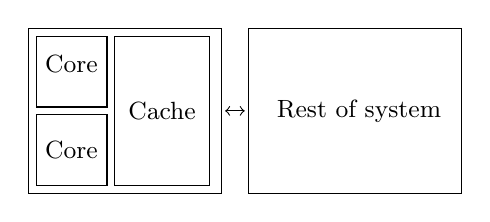
\begin{tikzpicture}
\draw (-0.5, -0.5) rectangle ++(0.9, 0.9);
\draw (-0.05, 0.05) node {\small Core};

\draw (-0.5, -1.5) rectangle ++(0.9, 0.9);
\draw (-0.05, -1.05) node {\small Core};

\draw (0.5, -1.5) rectangle ++(1.2, 1.9);
\draw (1.1, -.55) node {\small Cache};

\draw (-0.6, -1.6) rectangle ++(2.45, 2.1);

\draw (2.2, -1.6) rectangle ++(2.7, 2.1);
\draw (3.6, -0.55) node {\small Rest of system};

\draw[<->] (1.9, -0.55) -- (2.15, -0.55);
\end{tikzpicture}
\end{center}
\vspace*{-1em}
\hfill (credit: \emph{Multicore Application Programming}, p. 5)

This above Symmetric Multithreading (SMP) design is especially good for the 1:1 threading model. In
this case, the design of the cores don't need to change much, but they
still need to communicate with each other and the rest of the system.

Or, we can have a design that works well for the N:1 model:
\begin{center}
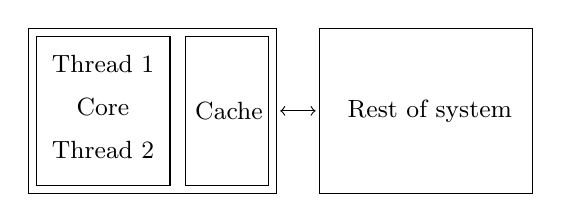
\begin{tikzpicture}
\draw (-1.4, -1.5) rectangle ++(1.7, 1.9);
\draw (-0.55, 0.05) node {\small Thread 1};
\draw (-0.55, -1.05) node {\small Thread 2};
\draw (-0.55, -0.5) node {\small Core};

\draw (0.5, -1.5) rectangle ++(1.05, 1.9);
\draw (1.05, -.55) node {\small Cache};

\draw (-1.5, -1.6) rectangle ++(3.15, 2.1);

\draw (2.2, -1.6) rectangle ++(2.7, 2.1);
\draw (3.6, -0.55) node {\small Rest of system};

\draw[<->] (1.7, -0.55) -- (2.15, -0.55);
\end{tikzpicture}
\end{center}

One would expect that executing two threads on one core might
mean that each thread would run more slowly. It depends on the instruction
mix. If the threads are trying to access the same resource, then each
thread would run more slowly. If they're doing different things, there's 
potential for speedup.

Finally, it's possible to both use multiple cores and put multiple threads
onto one core, as in the M:N model:

\begin{center}
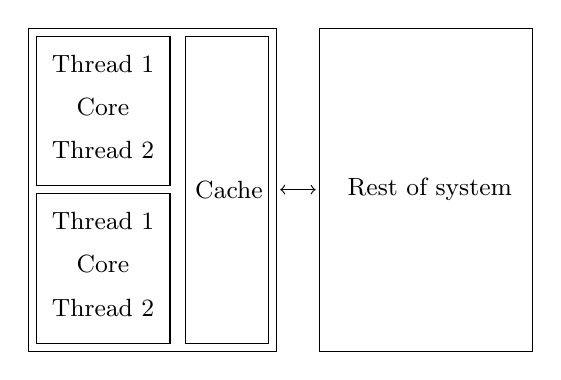
\begin{tikzpicture}

 \draw (-1.4, -1.5) rectangle +(1.7, 1.9);
 \draw (-1.4, -3.5) rectangle +(1.7, 1.9);

\foreach \y in {-2, 0}
{
 \draw (-0.55, 0.05) + (0, \y) node {\small Thread 1};
 \draw (-0.55, -1.05) + (0, \y) node {\small Thread 2};
 \draw (-0.55, -0.5) + (0, \y) node {\small Core};
}

\draw (0.5, -3.5) rectangle ++(1.05, 3.9);
\draw (1.05, -1.55) node {\small Cache};

\draw (-1.5, -3.6) rectangle ++(3.15, 4.1);

\draw (2.2, -3.6) rectangle ++(2.7, 4.1);
\draw (3.6, -1.55) node {\small Rest of system};

\draw[<->] (1.7, -1.55) -- (2.15, -1.55);
\end{tikzpicture}
\end{center}
Here we have four hardware threads; pairs of threads share hardware
resources. One example of a processor which supports chip multi-threading
(CMT) is the UltraSPARC T2, which has 8 cores, each of which supports 8 
threads. All of the cores share a common level 2 cache.

\paragraph{Non-SMP systems.} The designs we've seen above have been
more or less SMP designs; all of the cores are mostly alike.
A very non-SMP system is the Cell, which contains a PowerPC main core
(the PPE) and 7 Synergistic Processing Elements (SPEs), which are
small vector computers.


\paragraph{Non-Uniform Memory Access.}
In SMP systems, all CPUs have approximately the same access time for resources
(subject to cache misses). There are also NUMA, or Non-Uniform Memory Access,
systems out there. In that case, CPUs can access different resources at different
speeds. (Resources goes beyond just memory).

In this case, the operating system should schedule tasks on CPUs which
can access resources faster.  Since memory is commonly the bottleneck,
each CPU has its own memory bank.

\paragraph{Using CMT effectively.} Typically, a CPU will expose its
hardware threads using virtual CPUs.
In current hardware designs, each of the hardware threads has the same
performance. 

However, performance varies depending on context. In the above
example, two threads running on the same core will most probably run
more slowly than two threads running on separate cores, since they'd
contend for the same core's resources. Task switches between cores (or
CPUs!) are also slow, as they may involve reloading caches.

Solaris ``processor sets''
enable the operating system to assign processes to specific virtual CPUs,
while Linux's ``affinity'' keeps a process running on the same virtual CPU.
Both of these features reduce the number of task switches, and processor
sets can help reduce resource contention, along with Solaris's locality
groups.\footnote{Gove suggests that locality groups help reduce contention
for core resources, but they seem to help more with memory.}



\section*{Branch Prediction and Misprediction}

The compiler (and the CPU) take a look at code that results in branch instructions  such as loops, conditionals, or the dreaded \texttt{goto}\footnote{Which I still maintain is a swear word in C.}, and it will take an assessment of what it thinks is likely to happen. By default I think it's assumed that backward branches are taken and forward branches are not taken (but that may be wrong).  Well, how did we get here anyway?

In the beginning the CPUs and compilers didn't really think about this sort of thing, they would just come across instructions one at a time and do them and that was that. If one of them required a branch, it was no real issue. Then we had pipelining: the CPU would fetch the next instruction while decoding the previous one, and while executing the instruction before. That means if evaluation of an instruction results in a branch, we might go somewhere else and therefore throw away the contents of the pipeline. Thus we'd have wasted some time and effort. If the pipeline is short, this is not very expensive. But pipelines keep getting longer\ldots

So then we got to the subject of branch prediction. The compiler and CPU look at instructions on their way to be executed and analyze whether it thinks it's likely the branch is taken. This can be based on several things, including the recent execution history. If we guess correctly, this is great, because it minimizes the cost of the branch. If we guess wrong, we have to flush the pipeline and take the performance penalty.

The compiler and CPU's branch prediction routines are pretty smart. Trying to outsmart them isn't necessarily a good idea. It's possible to give \texttt{gcc} some hints: we say either something is likely or unlikely. 

 These hints tell the compiler some information about how it should predict. It will then arrange the instructions in such a way that, if the prediction is right, the instructions in the pipeline will be executed. But if we're wrong, then the instructions will have to be flushed.

From what I can tell, the core Rust team isn't super comfortable with the idea of exposing these kinds of internal-compiler things, but there is an implementation of the likely/unlikely concept. You can sort of use it, but it could break in the future, as an experimental feature. If you want the experimental features enabled, you have to be using nightly build of Rust and to specify the feature at the top of your source file (e.g., \texttt{\#![feature(core\_intrinsics)]})

Do they work? Here's a sample program to find out. I'll first test it with no hint, then putting \texttt{likely()} around the if condition, and then \texttt{unlikely()}, and show you the results.

\begin{lstlisting}[language=Rust]
fn f(a: i32) -> i32 {
    a
}

fn main() {
    let size = 100000;
    let large_vector = vec![0; size];
    let mut m1 = 0;
    let mut m2 = 0;

    for _j in 0..1000 {
        for k in 0..size {
            if *large_vector.get(k).unwrap() == 0 {
                m1 = f(m1 + 1)
            } else {
                m2 = f(m2 + 1)
            }
        }
    }
    println!("m1 = {}; m2 = {}", m1, m2);
}
\end{lstlisting}

And the results:
\begin{verbatim}
No hint at all:
  Time (mean +/- ?):      6.657 s +/-  0.144 s    [User: 6.614 s, System: 0.029 s]
  Range (min ... max):    6.413 s ...  6.905 s    10 runs
  
Likely:
  Time (mean +/- ?):      6.762 s +/-  0.175 s    [User: 6.729 s, System: 0.028 s]
  Range (min ... max):    6.590 s ...  7.200 s    10 runs

Unlikely:
  Time (mean +/- ?):      6.943 s +/-  0.200 s    [User: 6.893 s, System: 0.033 s]
  Range (min ... max):    6.732 s ...  7.309 s    10 runs
\end{verbatim}

Looks like hints don't help very much in this program at all. They made it marginally worse, not better. And getting it wrong comes with a penalty, too. This program might not be the ideal test case for hints, in that there might be a different scenario where the hints have a positive impact. However, we have at least established that hints aren't always a benefit, even if we know we're right. Under a lot of circumstances then, it's probably best just to leave it alone, unless we're really, really, really sure. 

Conclusion: it's hard to outsmart the compiler. Maybe it's better not to try.

\subsection*{How does branch prediction work, anyway?}
We can write software. The hardware will make it fast. If we understand the hardware, we can understand when it has trouble making our software fast.

You've seen how branch prediction works in ECE 222. However, we'll talk about it today in the context of performance. Notes based on a transcript of a talk by Dan Luu~\cite{branchprediction}.

I want you to pick up two points from this discussion:
\vspace*{-1em}
\begin{itemize}[noitemsep]
\item how branch predictors work---this helps you understand some of the apparent randomness in your
execution times, and possibly helps you make your code more predictable; and,
\item applying a (straightforward) expected value computation to predict performance.
\end{itemize}

Let's consider the following assembly code:

\hspace*{2em} \begin{minipage}{.4\textwidth} \begin{lstlisting}
branch_if_not_equal x, 0, else_label
// Do stuff
goto end_label
else_label:
// Do things
end_label:
// whatever happens later
\end{lstlisting}
\end{minipage}

The {\tt branch} instruction may be followed by either ``stuff'' or ``things''.
The pipeline needs to know what the next instruction is, for instance to fetch it.
But it can't know the next instruction until it almost finishes executing the branch.
Let's look at some pictures, assuming a 2-stage pipeline.

With no prediction, we need to serialize:

\begin{center}
\begin{tabular}{c|c|c|c}
bne.1 & bne.2 \\ \hline
& & things.1 & things.2
\end{tabular}
\end{center}

\begin{minipage}{.49\textwidth}
Let's predict that ``things'' gets taken.
If our prediction is correct, we save time.

\begin{center}
\begin{tabular}{c|c|c}
bne.1 & bne.2 \\ \hline
& things.1 & things.2 \\
\\
\end{tabular}
\end{center}
\end{minipage} \hspace*{.02\textwidth} \begin{minipage}{.49\textwidth}
But we might be wrong and need to throw out the bad prediction.

\begin{center}
\begin{tabular}{c|c|c|c}
bne.1 & bne.2 \\ \cline{1-2}
& \sout{things.1} \\ \hline
& & stuff.1 & stuff.2
\end{tabular}
\end{center}
\end{minipage}

\paragraph{Cartoon model.} We need to quantify the performance.
For the purpose of this lecture, let's pretend that our pipelined
CPU executes, on average, one instruction per clock;
mispredicted branches cost 20 cycles, while correctly-predicted
branches cost 1 cycle. We'll also assume that the instruction
mix contains 80\% non-branches and 20\% branches. So we can predict
average cycles per instruction.

With no prediction (or always-wrong prediction):
\[
\mathrm{non\_branch\_\%} \times 1 \mathrm{~cycle} + \mathrm{branch\_\%} \times 20 \mathrm{~cycles} = 4.8 \mathrm{~cycles}.
\]
With perfect branch prediction:
\[
\mathrm{non\_branch\_\%} \times 1 \mathrm{~cycle} + \mathrm{branch\_\%} \times 1 \mathrm{~cycle} = 1 \mathrm{~cycle}.
\]
So we can make our code run 4.8$\times$ faster with branch prediction!

\paragraph{Predict taken.} What's the simplest possible thing? We can
predict that a branch is always taken. (Loop branches, for instance,
account for many of the branches in an execution, and are often taken.)
If we got 70\% accuracy, then our cycles per instruction would be:
\[
(0.8 + 0.7 \times 0.2) \times 1 \mathrm{~cycle} + (0.3 \times 0.2) \times 20 \mathrm{~cycles} = 2.14 \mathrm{~cycles}.
\]
The simplest possible thing already greatly improves the CPU's average throughput.

\paragraph{Backwards taken, forwards not taken (BTFNT).}
Let's leverage that observation about loop branches to do better.
Loop branches are, by definition, backwards (go back to previous
code). So we can design a branch predictor which predicts ``taken''
for backwards and ``not taken'' for forwards. The compiler can then
use this information to encode what it thinks about forwards branches
(that is, making the not-taken branch the one it thinks is more likely).
Let's say that this might get us to 80\% accuracy. \[
(0.8 + 0.8 \times 0.2) \times 1 \mathrm{~cycle} + (0.2 \times 0.2) \times 20 \mathrm{~cycles} = 1.76 \mathrm{~cycles}.
\]
The PPC 601 (1993) and 603 used this scheme.

\paragraph{Going dynamic: using history for branch prediction.}
So far, we will always make the same prediction at each branch---known as a
\emph{static} scheme. But we can do better by using what recently happened to
improve our predictions. This is particularly important when program execution
contains distinct phases, with distinct behaviours.
We therefore move to \emph{dynamic} schemes.

Once again, let's start with the simplest possible thing. For every branch,
we record whether it was taken or not last time it executed (a 1-bit scheme).
Of course, we can't store all branches. So let's use the low 6 bits of the address
to identify branches. Doing so raises the prospect of \emph{aliasing}:
different branches (with different behaviour) map to the same spot in the table.

We might get 85\% accuracy with such a scheme.
\[
(0.8 + 0.85 \times 0.2) \times 1 \mathrm{~cycle} + (0.15 \times 0.2) \times 20 \mathrm{~cycles} = 1.57 \mathrm{~cycles}.
\]

At the cost of more hardware, we get noticeable performance improvements. The DEC EV4 (1992) and
MIPS R8000 (1994) used this one-bit scheme.

\paragraph{Two-bit schemes.}
What if a branch is almost always taken but occasionally not taken (e.g. TTTTTTNTTTT)?
We get penalized twice
for that misprediction: once when we mispredict the not taken, and once when we mispredict the
next taken. So, let's store whether a branch is ``usually'' taken, using a so-called
2-bit saturating counter.

Every time we see a taken branch, we increment the counter for that
branch; every time we see a not-taken branch, we decrement. Saturating
means that we don't overflow or underflow. We instead stay at 11 or
00, respectively.

If the counter is 00 or 01, we predict ``not taken''; if it is 10 or
11, we predict ``taken''.

With a two-bit counter, we can have fewer entries at the same size, but they'll do better.
It would be reasonable to expect 90\% accuracy.
\[
(0.8 + 0.9 \times 0.2) \times 1 \mathrm{~cycle} + (0.1 \times 0.2) \times 20 \mathrm{~cycles} = 1.38 \mathrm{~cycles}.
\]

This was used in a number of chips, from the LLNL S-1 (1977) through the Intel Pentium (1993).

\paragraph{Two-level adaptive, global.}
We're still not taking patterns into account. Consider the following {\tt for} loop.
\begin{lstlisting}[language=C]
for (int i = 0; i < 3; ++i) {
  // code
}
\end{lstlisting}
The last three executions of the branch determine the next direction:
\begin{verbatim}
 TTT => N
 TTN => T
 TNT => T
 NTT => T
\end{verbatim}
Let's store what happened the last few times we were at a particular address---the
\emph{branch history}. From a branch address and history, we derive an index, which
points to a table of 2-bit saturating counters. What's changed from the two-bit scheme
is that the history helps determine the index and hence the prediction.

After we take a branch, we add its direction to the history, so that the next lookup
maps to a different table entry.

This scheme might give something like 93\% accuracy.
\[
(0.8 + 0.93 \times 0.2) \times 1 \mathrm{~cycle} + (0.07 \times 0.2) \times 20 \mathrm{~cycles} = 1.27 \mathrm{~cycles}.
\]

The Pentium MMX (1996) used a 4-bit global branch history.

\paragraph{Two-level adaptive, local.}
The change here is that the CPU keeps a separate history for each branch.
So the branch address determines which branch history gets used.
We concatenate the address and history to get the index, which then points to a
2-bit counter again. We are starting to encounter diminishing returns, but we might
get 94\% accuracy:
\[
(0.8 + 0.94 \times 0.2) \times 1 \mathrm{~cycle} + (0.06 \times 0.2) \times 20 \mathrm{~cycles} = 1.23 \mathrm{~cycles}.
\]

The Pentium Pro (1996), Pentium II (1997) and Pentium III (1999) use this.

\paragraph{gshare.}
Instead of concatenating the address and history, we can xor them. This allows
us to use more bits for both the history and address. This keeps the accuracy the same,
but simplifies the design.

\paragraph{Other predictors.} We can build (and people have built) more sophisticated predictors.
These predictors could, for instance, better handle aliasing, where
different branches/histories map to the same index in the table. But we'll stop here.

\paragraph{Summary of branch prediction.} We can summarize as follows.
Branch prediction enables pipelining and hence increased performance.
We can create a model to estimate just how critical branch prediction
is for modern processors. Fortunately, most branches are predictable
now. Aliasing (multiple branches mapping to the same entry in a
prediction table) can be a problem, but processors are pretty good at
dealing with that too.

\section*{Side-channel attacks}
There's been a lot happening lately in terms of exploiting the hardware of CPU architectures to get access to privileged data, and unfortunately these things have performance implications!

\subsection*{Cache Attacks}
In early 2018, the Spectre~\cite{Kocher2018spectre} and Meltdown~\cite{Lipp2018meltdown} attacks were disclosed. These attacks leverage performance features of modern CPUs to break process isolation guarantees---in principle, a process shouldn't be able to read memory that belongs to the kernel or to other processes.

The concept of cache side-channel attacks has been known for a while. If an attacker can get some memory loaded into the cache, then it can extract that memory using a cache side-channel attack.

Spectre and Meltdown can cause privileged memory to be loaded into the cache, and then extracted using a cache side-channel attack. We'll talk about Spectre (variant 2), since it attacks branch prediction in particular. My explanation follows~\cite{masters18:_what_meltd_spect} by Jon Masters of RedHat. However, you should now have enough background to follow the Google Project Zero description at~\cite{horn18:_readin}.

We know that at a branch, the CPU will start speculatively executing code at the inferred target of the branch. To exploit this vulnerability, the attack code convinces the CPU to speculatively execute code of its choice. The speculatively-executed attack code reads secret data (e.g. from the hypervisor kernel) and puts it in the cache. Once the data is in the cache, the attack proceeds by extracting the data from the cache.

Unfortunately, the only mitigation thus far involved additional security measures (in hardware and software) that unfortunately result in lower performance in program execution.

\subsection*{Hyperthreading attacks}
Multiprocessor (multicore) processors have some hardware that tries to keep the data consistent between different pipelines and caches (as we saw in the video). More processors, more threads means more work is necessary to keep these things in order. We will discuss cache coherence soon, but about hyperthreading... it turns out this is vulnerable too.

Remember that in hyperthreading, two threads are sharing the same execution core. That means they have hardware in common. Because of this, a thread can figure out what the other thread is doing by noticing its cache accesses and by timing how long it takes to complete operations. This is like sitting next to someone who's taking a multiple choice exam and noticing what answers they are choosing by how long it takes them to move their pencil down the page to fill in the correct circle. Yes, you have to be running on the same CPU as the victim, but still... Yikes! 

Researchers discovered and published a paper~\cite{portsmash} detailing the attack and showing a practical implementation of it. In the practical example, a 384-bit secret key is (over time) completely stolen by another process. It seems likely that this will lead in the long term to slowdowns of existing hardware as Operating System patches will need to prevent threads from different processes from using the same core... And possibly the only long term solution is to not use hyperthreading at all... the performance implications of which are both obvious and significant.

\bibliographystyle{alphaurl}
\bibliography{459}


\end{document}
